\documentclass[dvipsnames]{standalone}

\usepackage[utf8]{inputenc}
\usepackage{tikz}
\usepackage{pgfplots}
\usepackage{pgfkeys}
\usetikzlibrary{
    calc,
    shadows.blur, 
    arrows, 
    arrows.meta, 
    shapes.arrows, 
    decorations.markings, 
    positioning
}

\pgfplotsset{compat=1.18} 

\colorlet{block}{SkyBlue!50}
\colorlet{thread-bg}{LimeGreen!50}
\colorlet{grid-bg}{RedOrange!60}


\def\blockwidth{3.6cm}
\def\blockheight{2.4cm}
\def\blockmargin{0.2cm}
\def\blocktextdepth{2cm}
\def\gridcols{3}
\def\gridrows{2}
\def\gridwidth{
    \blockmargin + \gridcols * (\blockwidth + \blockmargin)
}
\def\gridheight{
    \blockmargin + \gridrows * (\blockheight + \blockmargin) + 1cm
}
\def\threadmargin{\blockmargin}
\def\threadwidth{\blockwidth}
\def\threadheight{\blockheight}
\def\zoomblockcols{4}
\def\zoomblockrows{3}
\def\zoomblockwidth{
    \threadmargin + \zoomblockcols * (\threadwidth + \threadmargin)
}
\def\zoomblockheight{
    \threadmargin + \zoomblockrows * (\threadheight + \threadmargin) + 1cm
}
\def\gridtextdepth{\gridheight - 1cm}
\def\zoomblocktextdepth{\zoomblockheight-1cm}

\pgfdeclarelayer{background}
\pgfsetlayers{background,main} 

\begin{document}
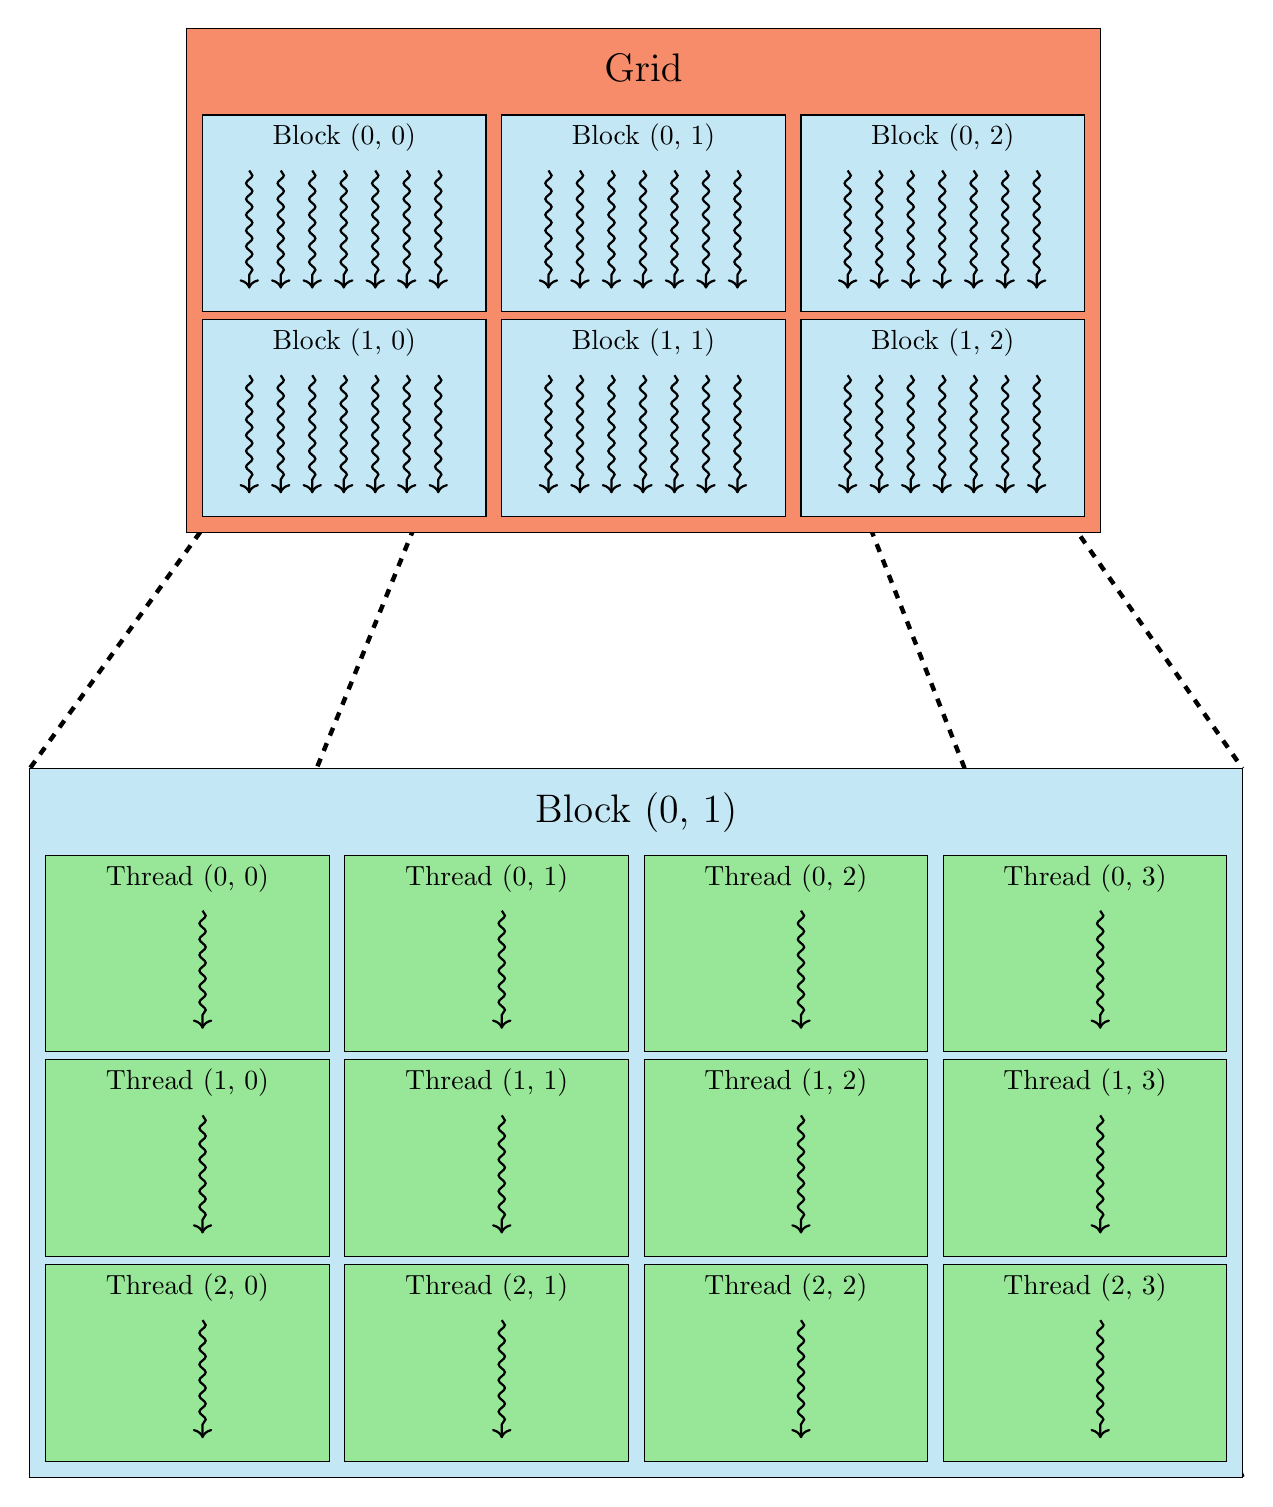
\begin{tikzpicture}[
    snake arrow/.style={->, thick,
        decorate,
        decoration={snake,
            amplitude=.4mm,
            segment length=2mm,
            post length=1mm}},
    zoom selection/.style={dashed, ultra thick},
    every node/.append style={anchor=south west},
    container/.style={
        draw, thin, align=center, text centered, rectangle
    },
    grid/.pic={
        \node[
            container, 
            minimum width=\gridwidth, 
            minimum height=\gridheight, 
            fill=grid-bg,
            text depth=\gridtextdepth,
        ] (grid) at (0, 0) {\Large Grid};
        \foreach \i[
            evaluate={
                \x=(\i-1)* (\blockwidth + \blockmargin)
            },
            evaluate={\blockidx=int(\i-1)}
        ] in {1,...,\gridcols} {
            \foreach \j[
                evaluate={
                    \y=(2-\j) * (\blockheight + \blockmargin)
                },
                evaluate={\blockidy=int(\j-1)}
            ] in {1,...,\gridrows} {
                \node[
                    container,
                    minimum width=\blockwidth, 
                    minimum height=\blockheight, 
                    fill=block,
                    text depth=\blocktextdepth
                ] (b\i\j) at (\blockmargin + \x, \blockmargin + \y) {Block (\blockidy, \blockidx)};
                \foreach \k in {-6,-4,...,6} {
                    \draw[thick] (2cm + \x+0.2 * \k cm, \y+2cm) edge[snake arrow] (2cm + \x+0.2 * \k cm, \y + 0.5cm);
                }
            }
        }    
    },
    zoomblock/.pic={
        \node[
            container,
            minimum width=\zoomblockwidth, 
            minimum height=\zoomblockheight, 
            fill=block,
            text depth=\zoomblocktextdepth,            
        ] at (0, 0) {\Large Block (0, 1)};        
        \foreach \i[
            evaluate={
                \x=(\i-1)* (\blockwidth + \blockmargin)
            },
            evaluate={\blockidx=int(\i-1)}
        ] in {1,...,\zoomblockcols} {
            \foreach \j[
                evaluate={
                    \y=(\zoomblockcols-\j-1) * (\blockheight + \blockmargin)
                },
                evaluate={\blockidy=int(\j-1)}
            ] in {1,...,\zoomblockrows} {
                \node[
                    container,
                    minimum width=\blockwidth, 
                    minimum height=\blockheight, 
                    fill=thread-bg,
                    text depth=\blocktextdepth
                ] at (\blockmargin + \x, \blockmargin + \y) {Thread (\blockidy, \blockidx)};
                \draw[thick] (2cm + \x+0.2cm, \y+2cm) edge[snake arrow] (2cm + \x+0.2cm, \y + 0.5cm);
            }
        }    
    }
]

\pic[local bounding box=grid] {grid}; 
\pic[below=12cm of grid, xshift=-7.8cm, local bounding box=zoomblock] {zoomblock};

\begin{pgfonlayer}{background}
    \draw[zoom selection] (b21.north west) -- (zoomblock.north west);
    \draw[zoom selection] (b21.south west) -- (zoomblock.south west);
    \draw[zoom selection] (b21.south east) -- (zoomblock.south east);
    \draw[zoom selection] (b21.north east) -- (zoomblock.north east);
\end{pgfonlayer}
\end{tikzpicture}
\end{document}